\documentclass{article}

\usepackage[utf8]{inputenc}
\usepackage[T1]{fontenc}
\usepackage{amsmath}
\usepackage{graphicx}
\usepackage{listings}
\usepackage{xcolor}
\usepackage{tcolorbox}

\title{Livrable 5}
\author{
Schicke Samuel, Burellier Loucas, Amberny Peran, \\
Krainik-Saul Vladimir, Barnouin Clement
}
\date{\today}

\begin{document}

\newtcolorbox[auto counter, number within=section]{configbox}[1]{
    colback=gray!10, % Fond bleu clair
    colframe=blue!50, % Bordure bleue
    sharp corners, % Coins carrés
    boxrule=0.75pt, % Épaisseur de la bordure
    fonttitle=\bfseries, % Titre en gras
    title={Fichier : \texttt{#1}}, % Affiche le nom du fichier
    fontupper=\ttfamily, % Police monospace pour le contenu
    left=5pt, right=5pt, top=5pt, bottom=5pt, % Marges internes
    before skip=10pt, after skip=10pt, % Espacement avant/après la box
}
\newtcolorbox{rootcommand}{
    colback=gray!10, % Fond gris clair
    colframe=gray!90, % Bordure grise
    sharp corners, % Coins carrés
    boxrule=0.5pt, % Épaisseur de la bordure
    fontupper=\ttfamily, % Police monospace
    left=3pt, right=3pt, top=3pt, bottom=3pt, % Marges internes
    %fit to text,
    %boxrule=0pt,
    halign=flush left,
    before upper={\textcolor{gray!70}{\textbf{\#  }}},
    before skip=5pt, after skip=5pt, % Espacement avant/après la boxS
}
\newtcolorbox{command}{
    colback=gray!10, % Fond gris clair
    colframe=gray!90!green, % Bordure grise
    sharp corners, % Coins carrés
    boxrule=0.5pt, % Épaisseur de la bordure
    fontupper=\ttfamily, % Police monospace
    left=3pt, right=3pt, top=3pt, bottom=3pt, % Marges internes
    halign=flush left,
    before upper={\textcolor{green!70!black}{\textbf{\$  }}},
    before skip=5pt, after skip=5pt, % Espacement avant/après la boxS
}

\include{bav4_style_file}

\maketitle


\section{Introduction}
MiniCoffee est un groupe français spécialiste de l’univers du café, connu notamment pour ses machines à café en libre service. Pour l’année 2025, l’entreprise souhaite mettre à jour son infrastructure réseau interne en ajoutant : 
\begin{itemize}
    \item Divers serveurs d’utilité interne pour les employés et l'équipe informatique;
    \item Un réseau invité pour permettre à ses fournisseurs d’utiliser du matériel informatique sur place;
    \item Divers serveurs accessibles en ligne (site Web, serveur DNS public);
    \item Une meilleure communication entre ses machines à café et son infrastructure, qui a été un des points faibles de l’entreprise ces dernières années.
\end{itemize}
Pour cette tâche, MiniCoffee a fait appel à BAV4, notre équipe d’étudiants de l’IUT2 Informatique de Grenoble.

\section{Architecture}
L'architecture de notre réseau n'a pas énormément changé. 
Les seules modifications apportées au réseau sont : 
\begin{itemize}
    \item Passage d'un LAN à un VLAN pour une meilleure segmentation du réseau.
    \item Les adresses IP internes se terminent par 1XX.
    \item Les adresses IP externes se terminent par XX.
\end{itemize}

\begin{figure}
    \centering
    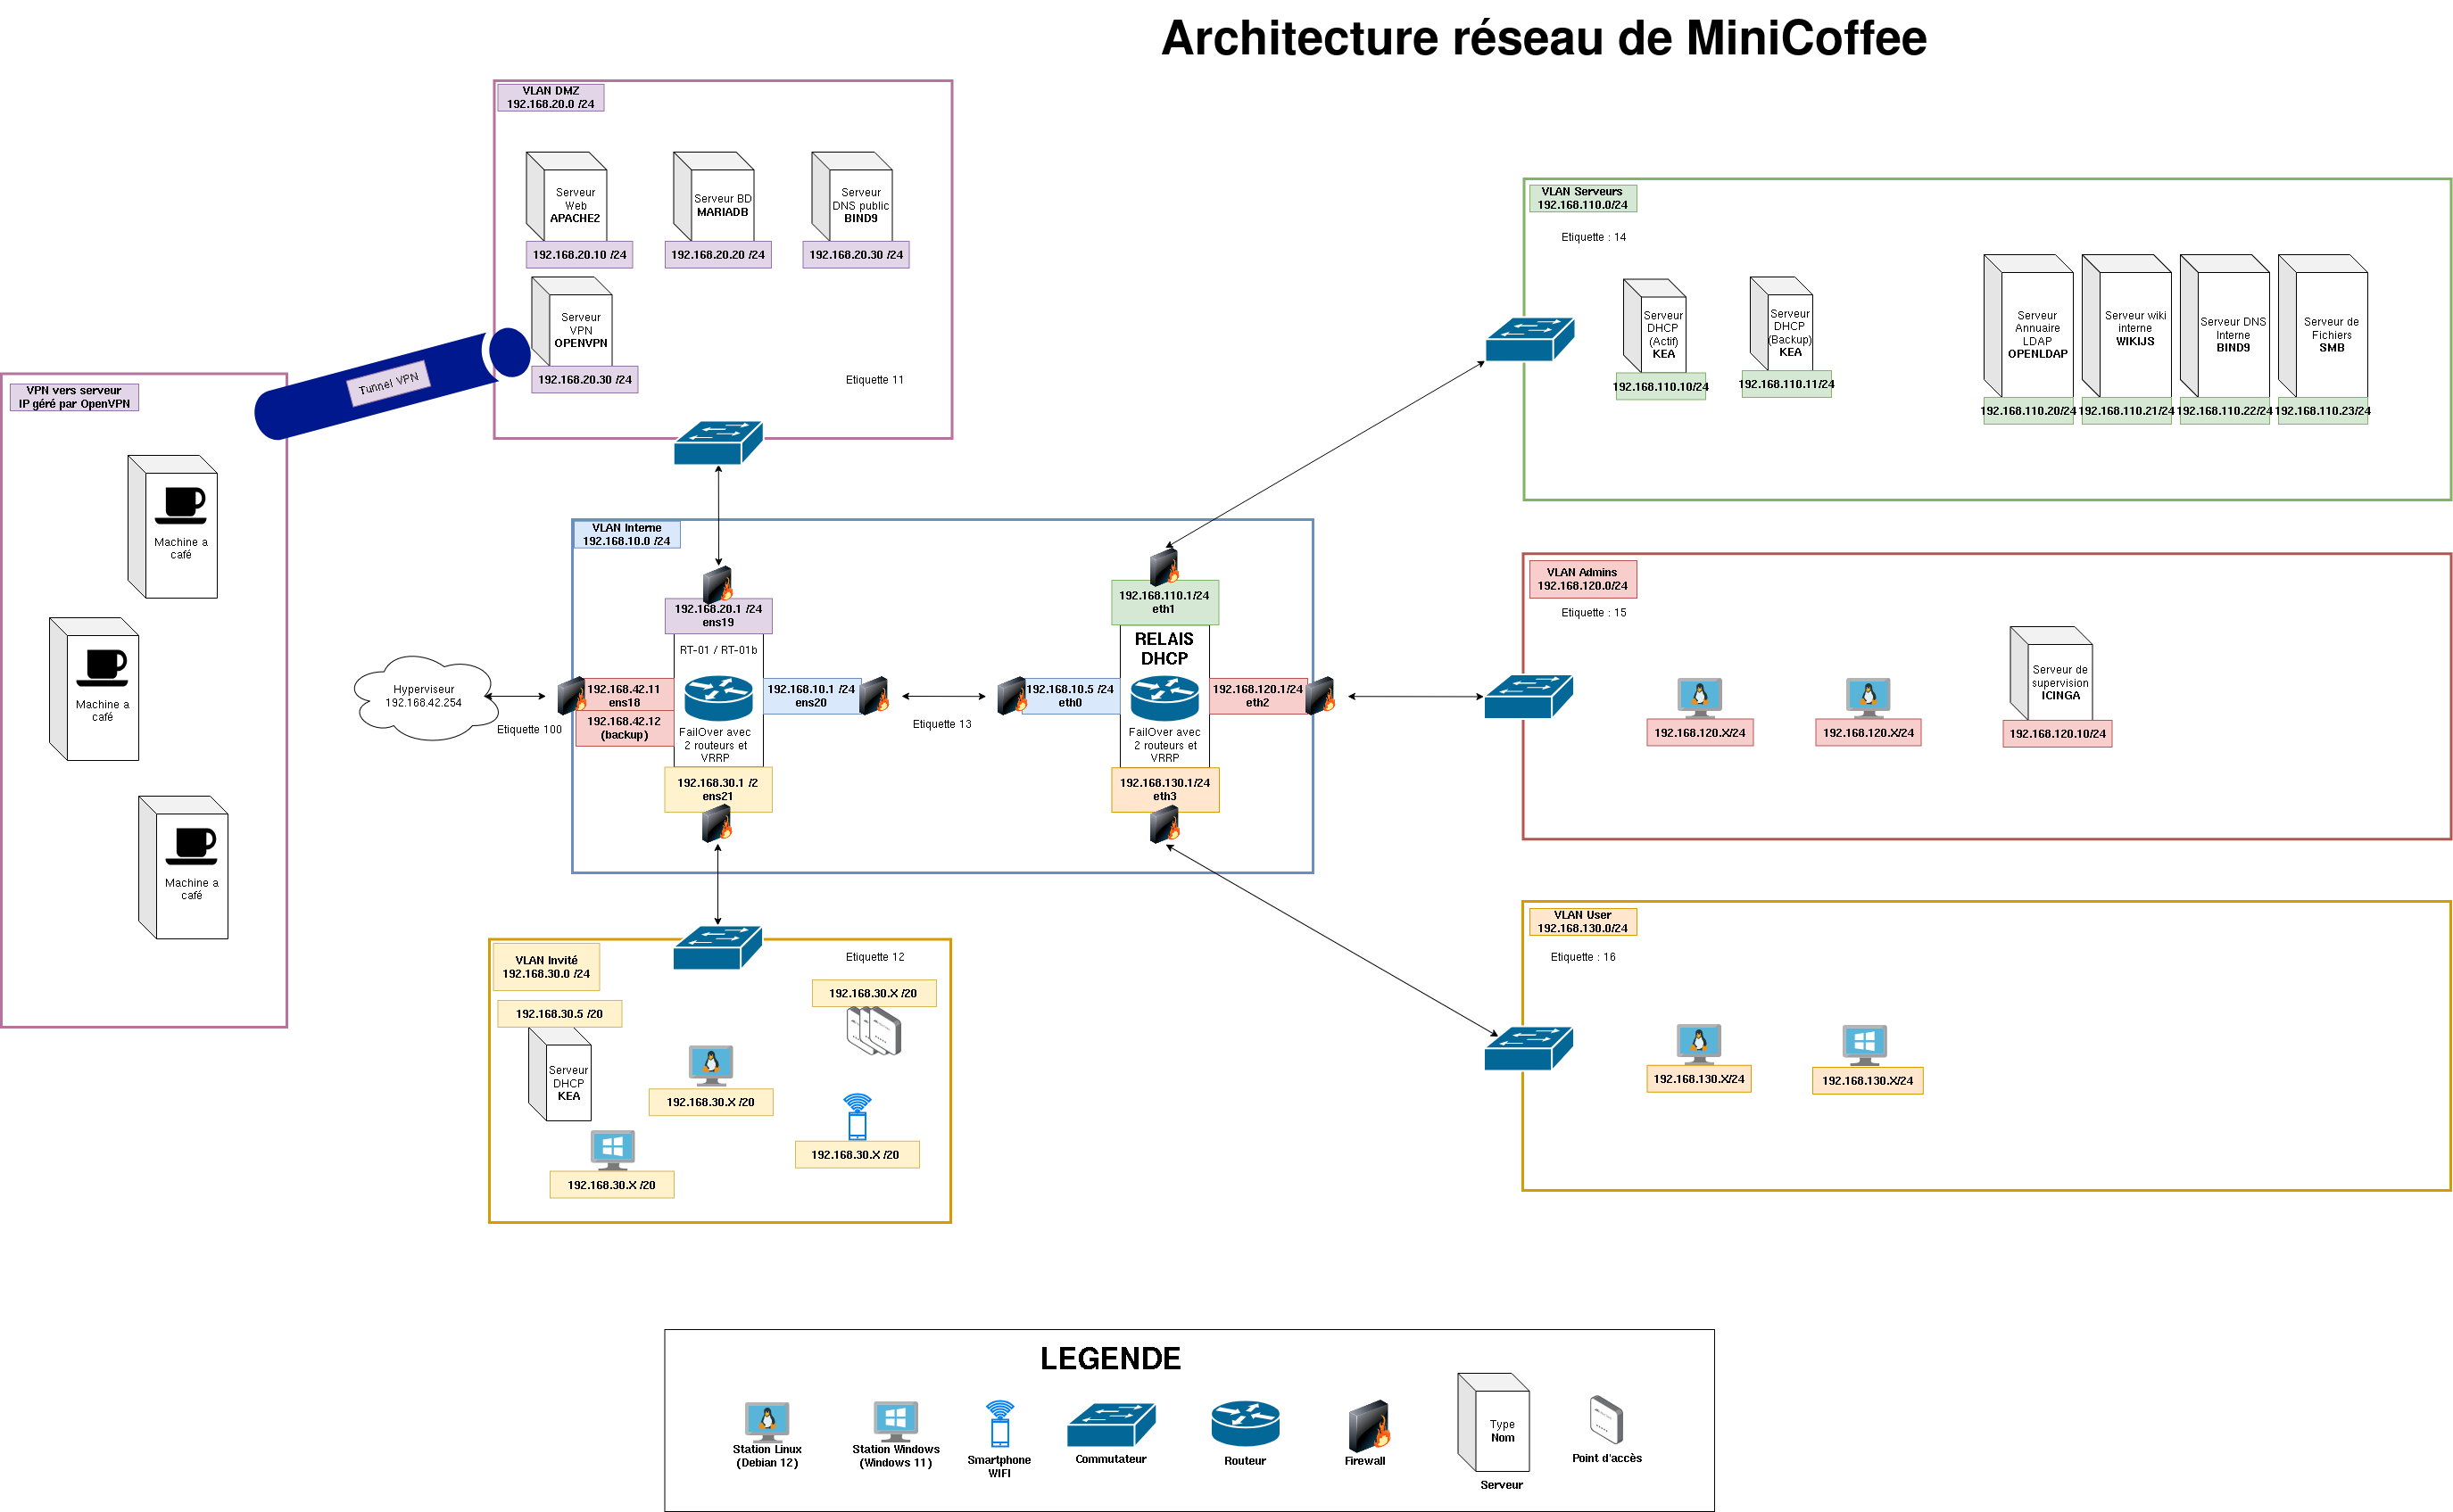
\includegraphics[width=1.2\textwidth, trim=0 0 0 2.3cm, clip]{../assets/Architecture.drawio.png}
    \caption{Architecture réseau de MiniCoffee}
\end{figure}

\clearpage

\section{Ressources Matérielles utilisées}
Actuellement, notre infrastructure réseau comprend un total de 9 machines actives, chacune jouant un rôle spécifique dans notre environnement.
\\

En ce qui concerne le stockage, nous allouons entre 3 et 5 Go d’espace disque par machine, en fonction de leurs besoins en ressources et des tâches qu’elles doivent accomplir. Plus précisément :
\begin{itemize}
    \item Les machines nécessitant le moins de ressources se voient attribuer 3 Go de stockage, ce qui est suffisant pour assurer leur bon fonctionnement sans surconsommation d’espace.
    \item Les machines les plus sollicitées, qui traitent des volumes de données plus importants ou exécutent des processus plus intensifs, bénéficient quant à elles de 5 Go de stockage afin de garantir des performances optimales.
\end{itemize}

En termes de mémoire vive (RAM), chaque machine de notre réseau dispose actuellement de 1 Go. Cette allocation permet de répondre aux besoins de nos applications tout en maintenant un bon équilibre entre performance et consommation de ressources.
\\

Nous surveillons régulièrement l’utilisation de la RAM et du stockage afin d’optimiser notre infrastructure si nécessaire et d’anticiper toute montée en charge.

\section{Installation et Configuration des éléments de l'infrastrucure}
On va détailler dans cette partie comment nous avons configuré les éléments de notre infrastructure réseau.
\subsection{Résaux Virtuel}

\subsection{Routeurs}
Tout d'abord, il faut configurer les interfaces de la machine qui va servir de routeur.

Il faut configurer le fichier \textbf{/etc/network/interfaces} pour attribuer les bonnes ip et CIDR pour chaque interface. Voici un explique de chaque paramètre que l’on peut mettre :

\newpage

\begin{itemize}
    \item Une première ligne avec la façon d’on l’interface s’active.
    \begin{itemize}
        \item \textbf{auto [nomInterface]} : Pour activer automatiquement au démarrage. Idéal pour les interfaces fixes, comme celles des serveurs.
        \item \textbf{allow-hotplug [nomInterface]} : Pour activer uniquement quand elle est détectée. Idéal pour les interfaces amovibles.
    \end{itemize}
    \item Une seconde qui définit sa configuration.
    \begin{itemize}
        \item \textbf{iface eth0 inet manual} : Interface n'a pas de configuration IP et doit être activé à la main
        \item \textbf{iface eth0 inet none} : Interface active mais sans configuration IP
        \item \textbf{iface [nomInterface] inet dhcp} : Utilise le DHCP pour l'attribution d'IP, ...
        \item \textbf{iface eth0 inet static} : Pour faire une configuration avec une IP statique
    \end{itemize}
    \item Ajout de paramètres pour la configuration de IP si configuration \textbf{static} :
    \begin{itemize}
        \item \textbf{address 192.168.100.14/24} : L'adresse IP static
        \item \textbf{gateway 192.168.100.1} : Le gateway
        \item \textbf{dns-nameservers 192.168.100.11 1.1.1.1} : Les DNS
        \item \textbf{dns-domain it-connect.local} : Le domaine DNS
        \item \textbf{metric 10} : La priorité de l'utilisation de cette interface. Plus la valeur est basse, plus la priorité est haute.
        \item \textbf{up ip addr add 192.168.100.15/24 dev [nomInterface]} : Si tu veux plusieurs adresses IP sur la même interface
        \item \textbf{mtu 9000} : MTU maximum
        \item \textbf{post-up ip route add 192.168.200.0/24 via 192.168.100.10} : Si la machine doit accéder à un réseau via une passerelle spécifique. Tout le trafic vers 192.168.200.0/24 passera via 192.168.100.10.
    \end{itemize}
\end{itemize}

Voici un fichier de configuration type pour un routeur avec plusieurs interface :

\begin{configbox}{/etc/network/interfaces}
    \begin{lstlisting}
        # Interface WAN (connectee a Internet)
        auto eth0
        iface eth0 inet dhcp
        mtu 1500  # Taille MTU standard
        # Interface LAN 1 
        (reseau interne 192.168.1.0/24)
        auto eth1
        iface eth1 inet static
            address 192.168.1.1/24
            gateway 192.168.1.254  # Facultatif, utilise uniquement si ce reseau doit 
            sortir par une autre route
            dns-nameservers 192.168.1.1 8.8.8.8
            dns-domain lan1.local
            mtu 9000  # Optimise pour les reseaux 
            locaux rapides

        # Interface LAN 2 
        (reseau interne 10.10.0.0/24)
        auto eth2
        iface eth2 inet static
            address 10.10.0.1/24
            mtu 9000  # Optimise pour un second 
            reseau local

        # Activation du routage entre les reseaux
    post-up echo 1 > /proc/sys/net/ipv4/ip_forward

        # Ajout de routes pour permettre aux 
        deux reseaux de communiquer entre eux
        # Ajout de routes pour permettre aux 
        deux reseaux de communiquer entre eux
    post-up ip route add 192.168.1.0/24 
    via 192.168.1.1 dev eth1
    post-up ip route add 10.10.0.0/24 
    via 10.10.0.1 dev eth2
    \end{lstlisting}
\end{configbox}

Une fois le fichier configurer, il redémarrer le service avec 
\begin{command}
sudo systemctl restart networking.service
\end{command}
Enfin, il faut activer l’interface avec 
\begin{command}
    ifup [nomInterface]
\end{command}
Ensuite il faut configurer les routes entre les réseaux
\\

Par défaut, une machine Linux ne fait pas passer n'importe quel paquet comme doit le faire un routeur. On doit donc activer cette fonctionnalité qui est sous la forme d'un option dans le fichier \textbf{/etc/sysctl.conf}, on devra y chercher la ligne suivante afin de la dé-commenter :

\begin{figure}[h]
    \centering
    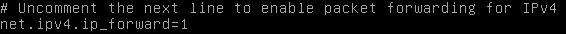
\includegraphics[width=1.2\textwidth]{../assets/image.png}
\end{figure}

Cette option active donc le **forwarding** (le "**relayage**" des paquets) d'une interface à une autre ou plus précisément d'un réseau à un autre. On pourra ensuite reloader notre sysctl :
\\

\begin{command}
    sysctl -p /etc/sysctl.conf
\end{command}

Mettre en place le NAT (fichier nft a executer) 
\begin{verbatim}
echo "1" > /proc/sys/net/ipv4/ip_forward
nft add table filtrage_nat
nft 'add chain filtrage_nat prerouting { type nat hook prerouting priority 0 ; }'
nft 'add chain filtrage_nat postrouting { type nat hook postrouting priority 0 ; }'
nft add rule filtrage_nat postrouting masquerade
\end{verbatim}

\subsection{Serveur DHCP}

\subsection{Serveur DNS}

\end{document}